\subsection{Clustering with Reduction vs Without}
\label{subsec:clustering-with-reduction-vs-without}

This section analyses the performance of clustering algorithms on two datasets, \textit{Mushroom} and \textit{Vowel}, with and without feature space reduction using three PCA methods:
\begin{itemize}
    \item PCA via SKLearn
    \item Our own implementation of PCA
    \item Kernel PCA via SKLearn
\end{itemize}
The Mean F-measure is used to evaluate performance.

Figures \ref{fig:clustering-results} show the F-measure scores for clustering with and without PCA. For each algorithm, the results are summarized as follows:

\begin{figure}[!h]
    \centering
    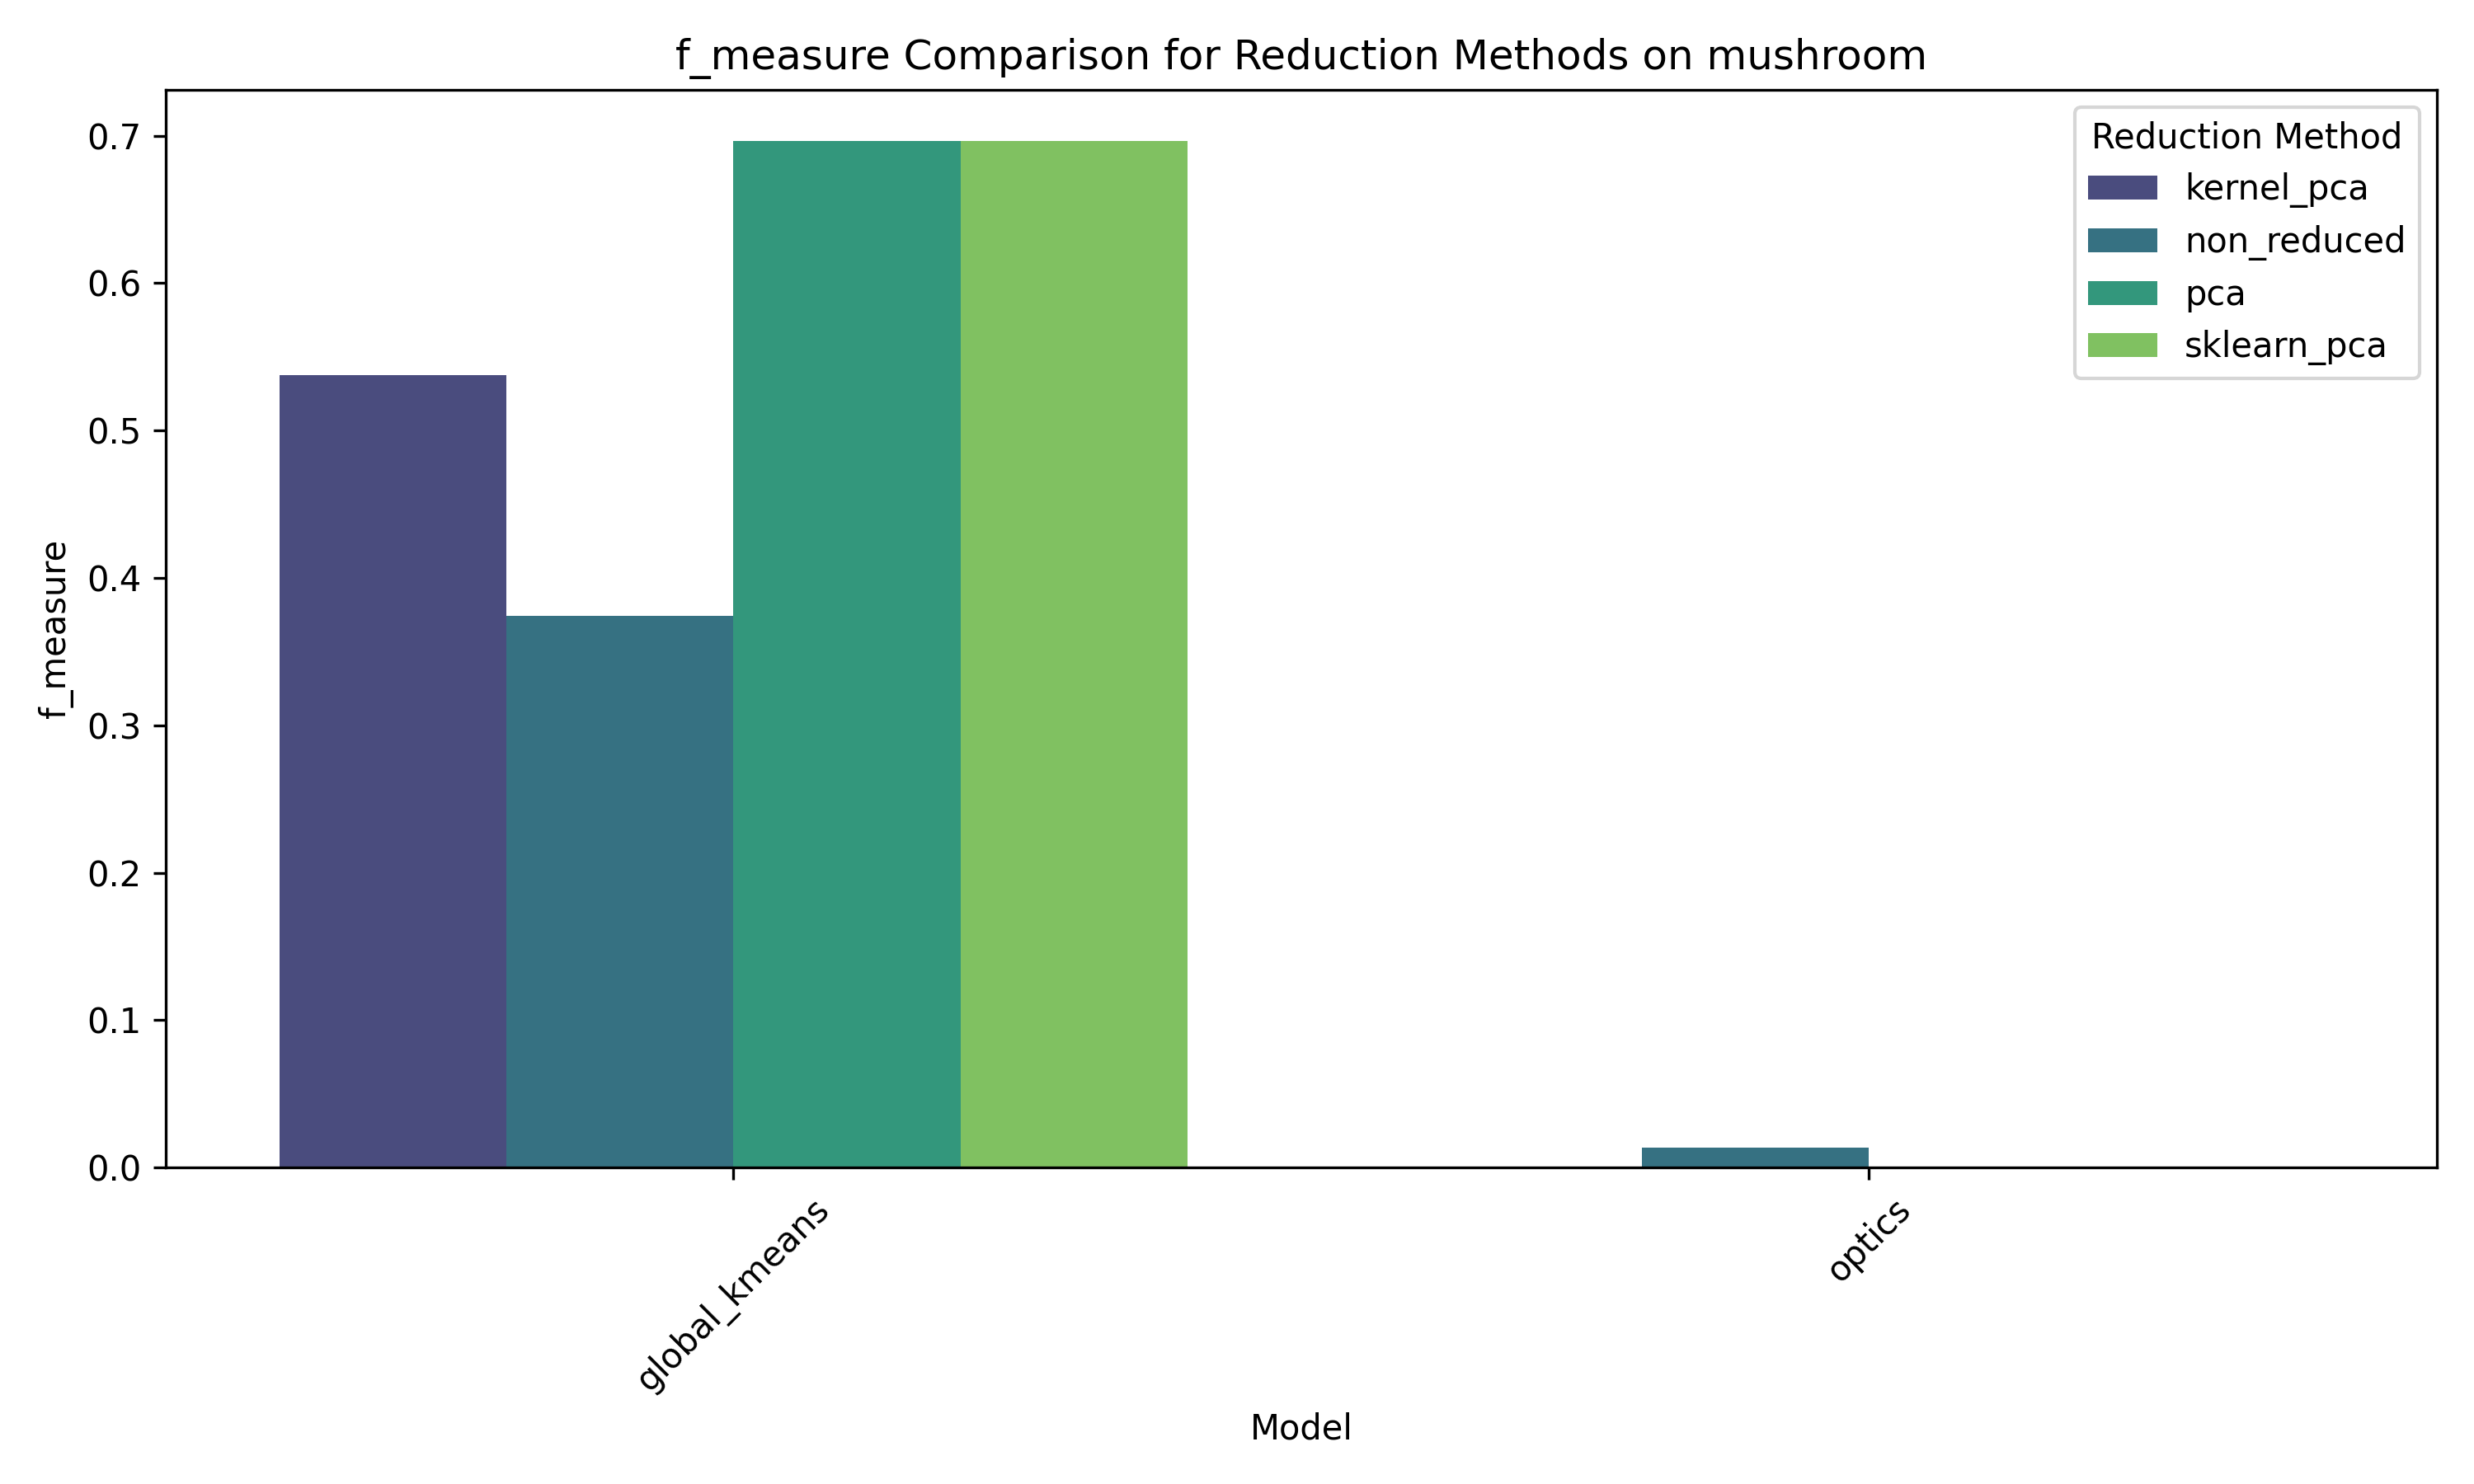
\includegraphics[width=0.45\textwidth]{figures/f_measure_comparison_mushroom.png}
    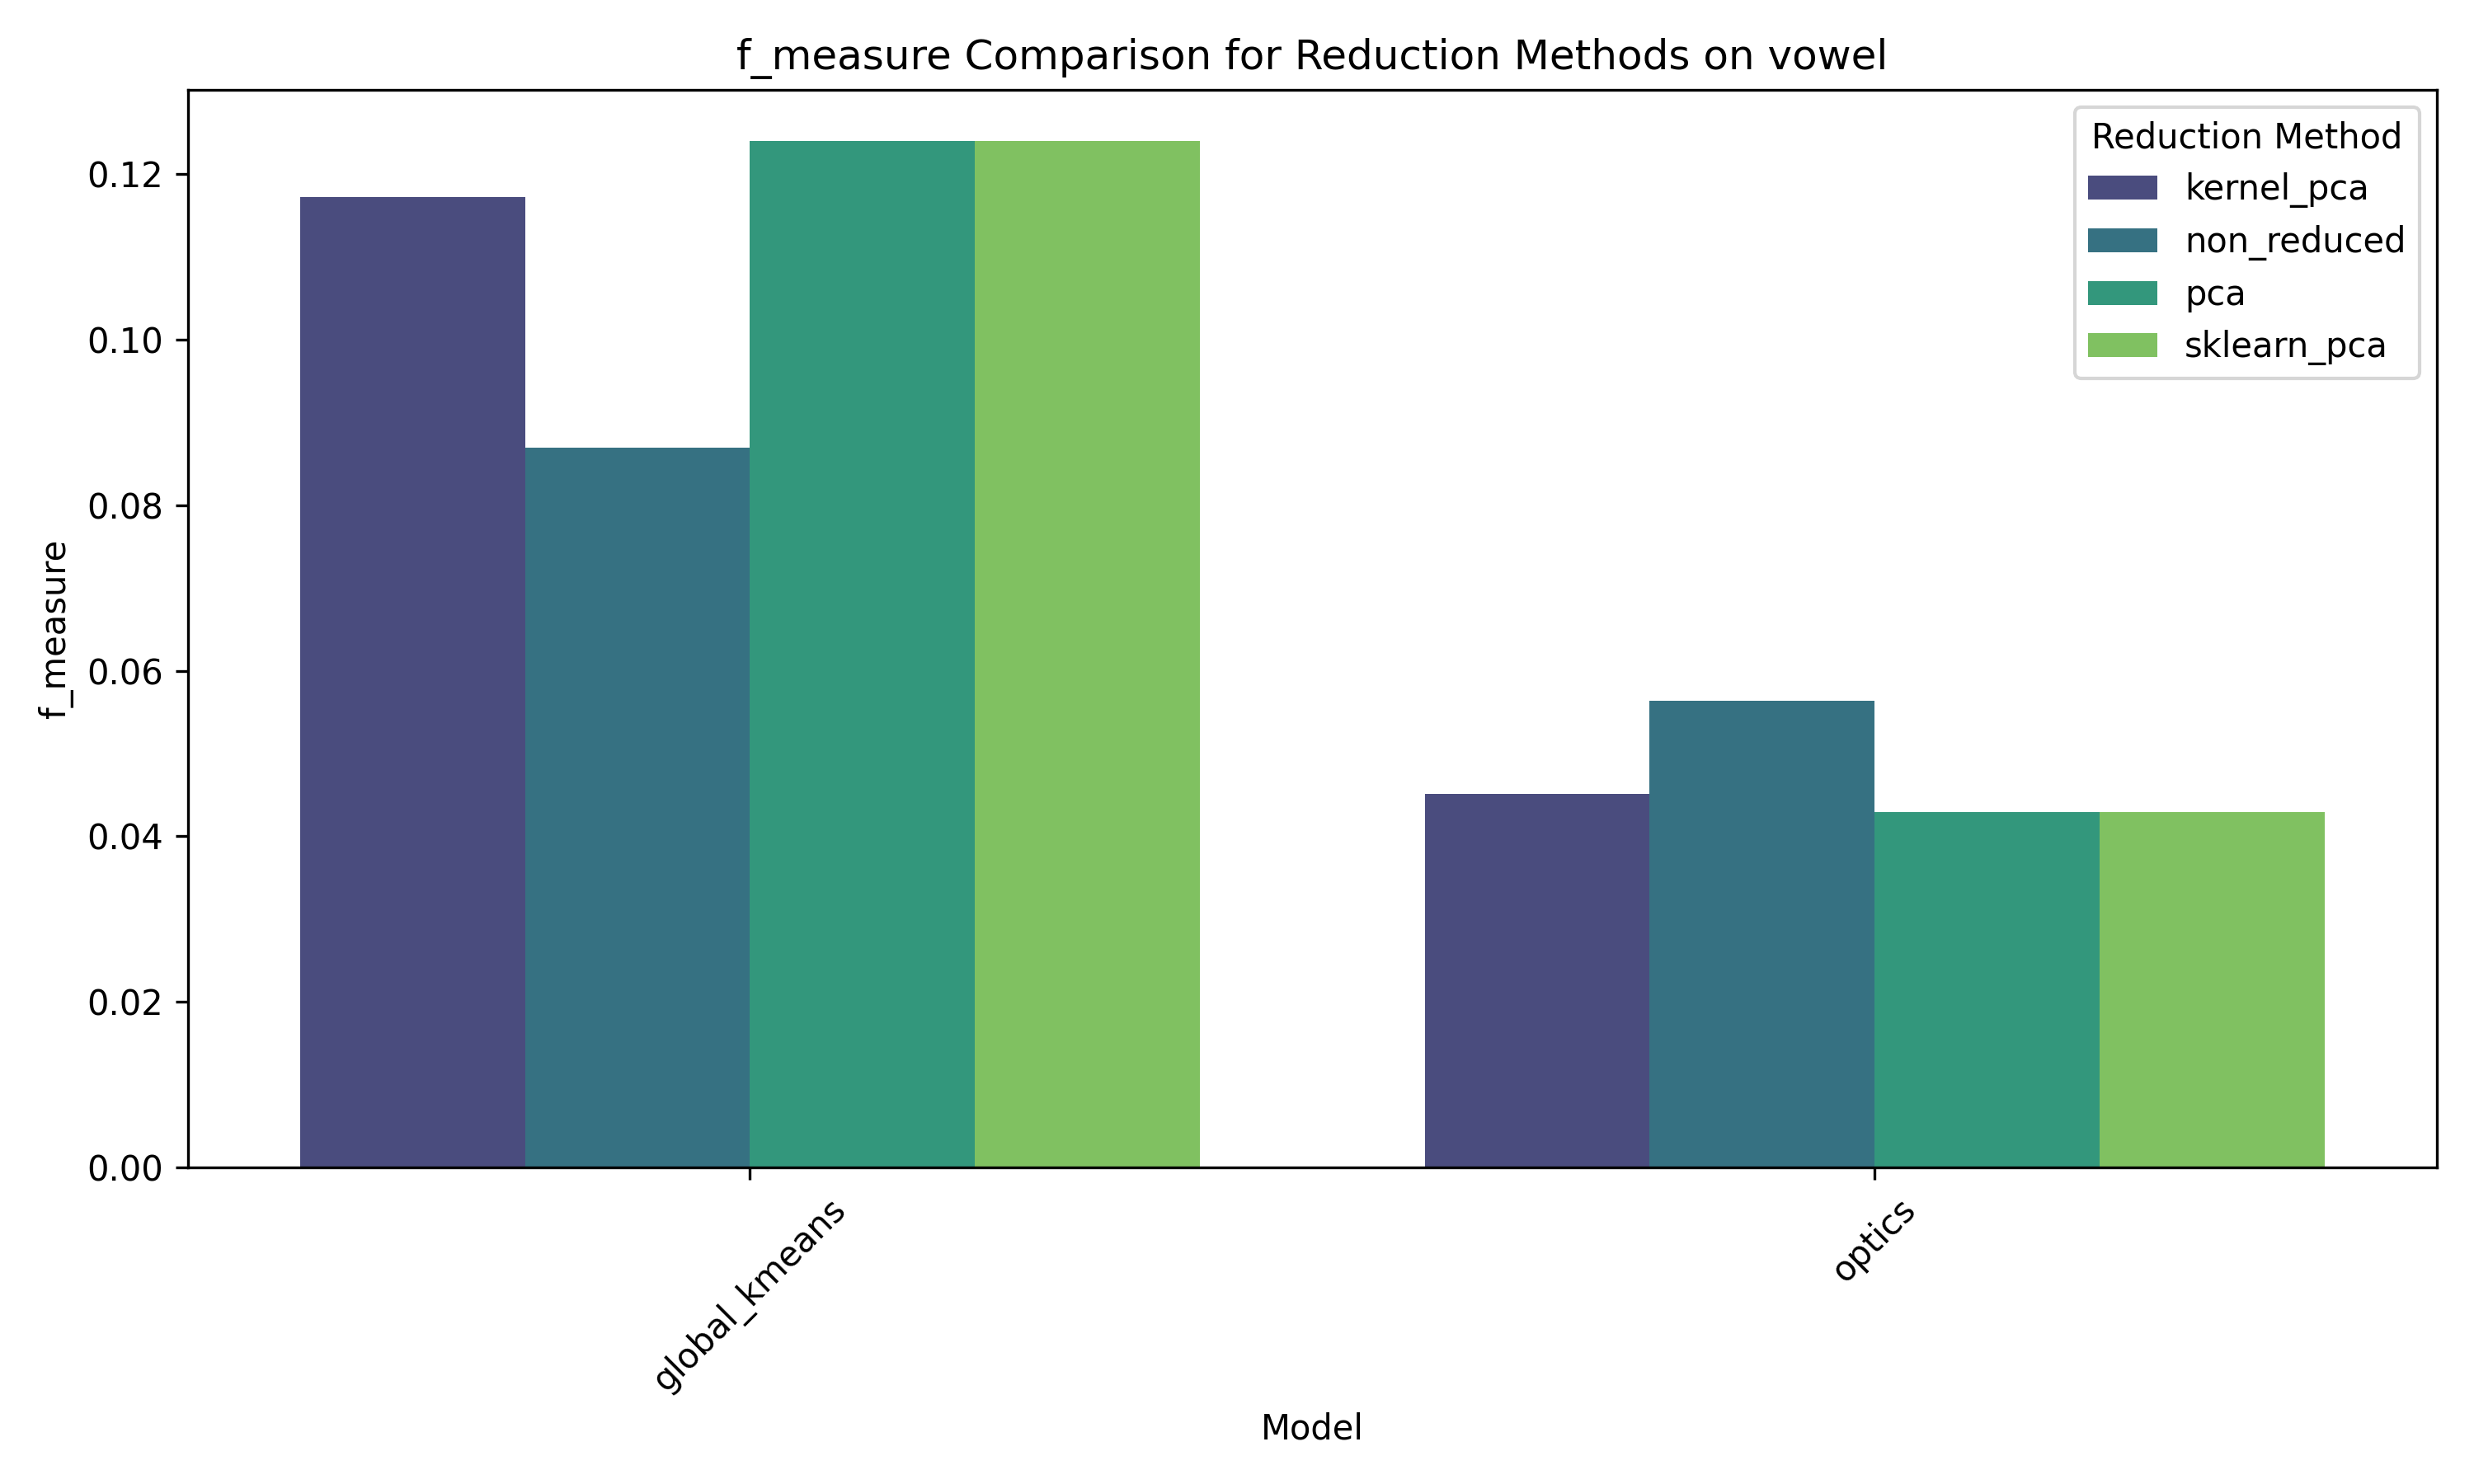
\includegraphics[width=0.45\textwidth]{figures/f_measure_comparison_vowel.png}
    \caption{Mean F-measure score with and without PCA for Mushroom (left) and Vowel (right) datasets.}
\label{fig:clustering-results}
\end{figure}

\paragraph{Global K-Means}
\begin{itemize}
    \item \textbf{Mushroom:} 
    \begin{itemize}
        \item Without PCA: F-measure $\approx 0.37$.
        \item With Kernel PCA: F-measure $\approx 0.53$.
        \item With our PCA and SKLearn PCA: F-measure $\approx 0.70$ (highest score).
    \end{itemize}
    \item \textbf{Vowel:} 
    \begin{itemize}
        \item Without PCA: F-measure $\approx 0.082$.
        \item With Kernel PCA: F-measure $\approx 0.11$.
        \item With our PCA and SKLearn PCA: F-measure $\approx 0.12$ (highest score).
    \end{itemize}
\end{itemize}

\paragraph{OPTICS}
\begin{itemize}
    \item \textbf{Mushroom:} 
    \begin{itemize}
        \item Without PCA: F-measure $\approx 0.02$.
        \item With any PCA method: F-measure drops to $\approx 0.0$.
    \end{itemize}
    \item \textbf{Vowel:} 
    \begin{itemize}
        \item Without PCA: F-measure $\approx 0.058$.
        \item With Kernel PCA: F-measure $\approx 0.043$.
        \item With our PCA and SKLearn PCA: F-measure $\approx 0.04$.
    \end{itemize}
\end{itemize}


From these results, PCA has a positive impact on \textit{Global K-Means}, where dimensionality reduction
highlights important features, improving clustering performance. Conversely, PCA degrades
the performance of \textit{OPTICS}, as its density-based approach is sensitive to
transformations that distort local density structures, which are critical for detecting clusters\cite{sepin2023comparisonclusteringalgorithmsstatistical}.

\autoref{tab:best_models_overall} highlights the best-performing models by dataset. \textit{Global K-Means}
consistently outperforms \textit{OPTICS}, achieving the highest F-measure scores. Similarly,
\autoref{tab:best_reduction_method_overall} shows that our PCA and SKLearn PCA yield the best
results overall for \textit{Global K-Means}, while OPTICS performs worse than \textit{Global K-Means} in all cases.


\begin{table*}[ht!]
\caption{Best Performing Models by Dataset (Based on F-Measure)}
\label{tab:best_models_overall}
\begin{tabular}{llrrrrr}
Dataset & Model & F Measure & Ari & Chi & Dbi & Runtime (s) \\\midrule

hepatitis & global\_kmeans & 0.7122 & 0.2555 & 36.5479 & 1.9827 & 0.0625 \\
mushroom & kmeans & 0.9434 & 0.7881 & 1070.0670 & 2.6995 & 0.3844 \\
vowel & spectral\_clustering & 0.1701 & 0.0438 & 19.2650 & 4.8690 & 0.0268 \\
\end{tabular}
\end{table*}


\input{../data/5_metrics_tables/best_reduction_method_overall.tex}
